\documentclass[11pt]{article}

    \usepackage[breakable]{tcolorbox}
    \usepackage{parskip} % Stop auto-indenting (to mimic markdown behaviour)
    \usepackage[final]{pdfpages}
    \usepackage{iftex}
    \ifPDFTeX
    	\usepackage[T1]{fontenc}
    	\usepackage{mathpazo}
    \else
    	\usepackage{fontspec}
    \fi
\usepackage{sectsty}
\sectionfont{\centering}
\sectionfont{\centering\normalfont}
    % Basic figure setup, for now with no caption control since it's done
    % automatically by Pandoc (which extracts ![](path) syntax from Markdown).
    \usepackage{graphicx}
    % Maintain compatibility with old templates. Remove in nbconvert 6.0
    \let\Oldincludegraphics\includegraphics
    % Ensure that by default, figures have no caption (until we provide a
    % proper Figure object with a Caption API and a way to capture that
    % in the conversion process - todo).
    \usepackage{caption}
    \DeclareCaptionFormat{nocaption}{}
    \captionsetup{format=nocaption,aboveskip=0pt,belowskip=0pt}

    \usepackage{float}
    \floatplacement{figure}{H} % forces figures to be placed at the correct location
    \usepackage{xcolor} % Allow colors to be defined
    \usepackage{enumerate} % Needed for markdown enumerations to work
    \usepackage{geometry} % Used to adjust the document margins
    \usepackage{amsmath} % Equations
    \usepackage{amssymb} % Equations
    \usepackage{textcomp} % defines textquotesingle
    % Hack from http://tex.stackexchange.com/a/47451/13684:
    \AtBeginDocument{%
        \def\PYZsq{\textquotesingle}% Upright quotes in Pygmentized code
    }
    \usepackage{upquote} % Upright quotes for verbatim code
    \usepackage{eurosym} % defines \euro
    \usepackage[mathletters]{ucs} % Extended unicode (utf-8) support
    \usepackage{fancyvrb} % verbatim replacement that allows latex
    \usepackage{grffile} % extends the file name processing of package graphics 
                         % to support a larger range
    \makeatletter % fix for old versions of grffile with XeLaTeX
    \@ifpackagelater{grffile}{2019/11/01}
    {
      % Do nothing on new versions
    }
    {
      \def\Gread@@xetex#1{%
        \IfFileExists{"\Gin@base".bb}%
        {\Gread@eps{\Gin@base.bb}}%
        {\Gread@@xetex@aux#1}%
      }
    }
    \makeatother
    \usepackage[Export]{adjustbox} % Used to constrain images to a maximum size
    \adjustboxset{max size={0.9\linewidth}{0.9\paperheight}}

    % The hyperref package gives us a pdf with properly built
    % internal navigation ('pdf bookmarks' for the table of contents,
    % internal cross-reference links, web links for URLs, etc.)
    \usepackage{hyperref}
    % The default LaTeX title has an obnoxious amount of whitespace. By default,
    % titling removes some of it. It also provides customization options.
    \usepackage{titling}
    \usepackage{longtable} % longtable support required by pandoc >1.10
    \usepackage{booktabs}  % table support for pandoc > 1.12.2
    \usepackage[inline]{enumitem} % IRkernel/repr support (it uses the enumerate* environment)
    \usepackage[normalem]{ulem} % ulem is needed to support strikethroughs (\sout)
                                % normalem makes italics be italics, not underlines
    \usepackage{mathrsfs}
    

    
    % Colors for the hyperref package
    \definecolor{urlcolor}{rgb}{0,.145,.698}
    \definecolor{linkcolor}{rgb}{.71,0.21,0.01}
    \definecolor{citecolor}{rgb}{.12,.54,.11}

    % ANSI colors
    \definecolor{ansi-black}{HTML}{3E424D}
    \definecolor{ansi-black-intense}{HTML}{282C36}
    \definecolor{ansi-red}{HTML}{E75C58}
    \definecolor{ansi-red-intense}{HTML}{B22B31}
    \definecolor{ansi-green}{HTML}{00A250}
    \definecolor{ansi-green-intense}{HTML}{007427}
    \definecolor{ansi-yellow}{HTML}{DDB62B}
    \definecolor{ansi-yellow-intense}{HTML}{B27D12}
    \definecolor{ansi-blue}{HTML}{208FFB}
    \definecolor{ansi-blue-intense}{HTML}{0065CA}
    \definecolor{ansi-magenta}{HTML}{D160C4}
    \definecolor{ansi-magenta-intense}{HTML}{A03196}
    \definecolor{ansi-cyan}{HTML}{60C6C8}
    \definecolor{ansi-cyan-intense}{HTML}{258F8F}
    \definecolor{ansi-white}{HTML}{C5C1B4}
    \definecolor{ansi-white-intense}{HTML}{A1A6B2}
    \definecolor{ansi-default-inverse-fg}{HTML}{FFFFFF}
    \definecolor{ansi-default-inverse-bg}{HTML}{000000}

    % common color for the border for error outputs.
    \definecolor{outerrorbackground}{HTML}{FFDFDF}

    % commands and environments needed by pandoc snippets
    % extracted from the output of `pandoc -s`
    \providecommand{\tightlist}{%
      \setlength{\itemsep}{0pt}\setlength{\parskip}{0pt}}
    \DefineVerbatimEnvironment{Highlighting}{Verbatim}{commandchars=\\\{\}}
    % Add ',fontsize=\small' for more characters per line
    \newenvironment{Shaded}{}{}
    \newcommand{\KeywordTok}[1]{\textcolor[rgb]{0.00,0.44,0.13}{\textbf{{#1}}}}
    \newcommand{\DataTypeTok}[1]{\textcolor[rgb]{0.56,0.13,0.00}{{#1}}}
    \newcommand{\DecValTok}[1]{\textcolor[rgb]{0.25,0.63,0.44}{{#1}}}
    \newcommand{\BaseNTok}[1]{\textcolor[rgb]{0.25,0.63,0.44}{{#1}}}
    \newcommand{\FloatTok}[1]{\textcolor[rgb]{0.25,0.63,0.44}{{#1}}}
    \newcommand{\CharTok}[1]{\textcolor[rgb]{0.25,0.44,0.63}{{#1}}}
    \newcommand{\StringTok}[1]{\textcolor[rgb]{0.25,0.44,0.63}{{#1}}}
    \newcommand{\CommentTok}[1]{\textcolor[rgb]{0.38,0.63,0.69}{\textit{{#1}}}}
    \newcommand{\OtherTok}[1]{\textcolor[rgb]{0.00,0.44,0.13}{{#1}}}
    \newcommand{\AlertTok}[1]{\textcolor[rgb]{1.00,0.00,0.00}{\textbf{{#1}}}}
    \newcommand{\FunctionTok}[1]{\textcolor[rgb]{0.02,0.16,0.49}{{#1}}}
    \newcommand{\RegionMarkerTok}[1]{{#1}}
    \newcommand{\ErrorTok}[1]{\textcolor[rgb]{1.00,0.00,0.00}{\textbf{{#1}}}}
    \newcommand{\NormalTok}[1]{{#1}}
    
    % Additional commands for more recent versions of Pandoc
    \newcommand{\ConstantTok}[1]{\textcolor[rgb]{0.53,0.00,0.00}{{#1}}}
    \newcommand{\SpecialCharTok}[1]{\textcolor[rgb]{0.25,0.44,0.63}{{#1}}}
    \newcommand{\VerbatimStringTok}[1]{\textcolor[rgb]{0.25,0.44,0.63}{{#1}}}
    \newcommand{\SpecialStringTok}[1]{\textcolor[rgb]{0.73,0.40,0.53}{{#1}}}
    \newcommand{\ImportTok}[1]{{#1}}
    \newcommand{\DocumentationTok}[1]{\textcolor[rgb]{0.73,0.13,0.13}{\textit{{#1}}}}
    \newcommand{\AnnotationTok}[1]{\textcolor[rgb]{0.38,0.63,0.69}{\textbf{\textit{{#1}}}}}
    \newcommand{\CommentVarTok}[1]{\textcolor[rgb]{0.38,0.63,0.69}{\textbf{\textit{{#1}}}}}
    \newcommand{\VariableTok}[1]{\textcolor[rgb]{0.10,0.09,0.49}{{#1}}}
    \newcommand{\ControlFlowTok}[1]{\textcolor[rgb]{0.00,0.44,0.13}{\textbf{{#1}}}}
    \newcommand{\OperatorTok}[1]{\textcolor[rgb]{0.40,0.40,0.40}{{#1}}}
    \newcommand{\BuiltInTok}[1]{{#1}}
    \newcommand{\ExtensionTok}[1]{{#1}}
    \newcommand{\PreprocessorTok}[1]{\textcolor[rgb]{0.74,0.48,0.00}{{#1}}}
    \newcommand{\AttributeTok}[1]{\textcolor[rgb]{0.49,0.56,0.16}{{#1}}}
    \newcommand{\InformationTok}[1]{\textcolor[rgb]{0.38,0.63,0.69}{\textbf{\textit{{#1}}}}}
    \newcommand{\WarningTok}[1]{\textcolor[rgb]{0.38,0.63,0.69}{\textbf{\textit{{#1}}}}}
    
    
    % Define a nice break command that doesn't care if a line doesn't already
    % exist.
    \def\br{\hspace*{\fill} \\* }
    % Math Jax compatibility definitions
    \def\gt{>}
    \def\lt{<}
    \let\Oldtex\TeX
    \let\Oldlatex\LaTeX
    \renewcommand{\TeX}{\textrm{\Oldtex}}
    \renewcommand{\LaTeX}{\textrm{\Oldlatex}}
    % Document parameters
    % Document title
    \title{Project 6}
    
    
    
    
    
% Pygments definitions
\makeatletter
\def\PY@reset{\let\PY@it=\relax \let\PY@bf=\relax%
    \let\PY@ul=\relax \let\PY@tc=\relax%
    \let\PY@bc=\relax \let\PY@ff=\relax}
\def\PY@tok#1{\csname PY@tok@#1\endcsname}
\def\PY@toks#1+{\ifx\relax#1\empty\else%
    \PY@tok{#1}\expandafter\PY@toks\fi}
\def\PY@do#1{\PY@bc{\PY@tc{\PY@ul{%
    \PY@it{\PY@bf{\PY@ff{#1}}}}}}}
\def\PY#1#2{\PY@reset\PY@toks#1+\relax+\PY@do{#2}}

\@namedef{PY@tok@w}{\def\PY@tc##1{\textcolor[rgb]{0.73,0.73,0.73}{##1}}}
\@namedef{PY@tok@c}{\let\PY@it=\textit\def\PY@tc##1{\textcolor[rgb]{0.25,0.50,0.50}{##1}}}
\@namedef{PY@tok@cp}{\def\PY@tc##1{\textcolor[rgb]{0.74,0.48,0.00}{##1}}}
\@namedef{PY@tok@k}{\let\PY@bf=\textbf\def\PY@tc##1{\textcolor[rgb]{0.00,0.50,0.00}{##1}}}
\@namedef{PY@tok@kp}{\def\PY@tc##1{\textcolor[rgb]{0.00,0.50,0.00}{##1}}}
\@namedef{PY@tok@kt}{\def\PY@tc##1{\textcolor[rgb]{0.69,0.00,0.25}{##1}}}
\@namedef{PY@tok@o}{\def\PY@tc##1{\textcolor[rgb]{0.40,0.40,0.40}{##1}}}
\@namedef{PY@tok@ow}{\let\PY@bf=\textbf\def\PY@tc##1{\textcolor[rgb]{0.67,0.13,1.00}{##1}}}
\@namedef{PY@tok@nb}{\def\PY@tc##1{\textcolor[rgb]{0.00,0.50,0.00}{##1}}}
\@namedef{PY@tok@nf}{\def\PY@tc##1{\textcolor[rgb]{0.00,0.00,1.00}{##1}}}
\@namedef{PY@tok@nc}{\let\PY@bf=\textbf\def\PY@tc##1{\textcolor[rgb]{0.00,0.00,1.00}{##1}}}
\@namedef{PY@tok@nn}{\let\PY@bf=\textbf\def\PY@tc##1{\textcolor[rgb]{0.00,0.00,1.00}{##1}}}
\@namedef{PY@tok@ne}{\let\PY@bf=\textbf\def\PY@tc##1{\textcolor[rgb]{0.82,0.25,0.23}{##1}}}
\@namedef{PY@tok@nv}{\def\PY@tc##1{\textcolor[rgb]{0.10,0.09,0.49}{##1}}}
\@namedef{PY@tok@no}{\def\PY@tc##1{\textcolor[rgb]{0.53,0.00,0.00}{##1}}}
\@namedef{PY@tok@nl}{\def\PY@tc##1{\textcolor[rgb]{0.63,0.63,0.00}{##1}}}
\@namedef{PY@tok@ni}{\let\PY@bf=\textbf\def\PY@tc##1{\textcolor[rgb]{0.60,0.60,0.60}{##1}}}
\@namedef{PY@tok@na}{\def\PY@tc##1{\textcolor[rgb]{0.49,0.56,0.16}{##1}}}
\@namedef{PY@tok@nt}{\let\PY@bf=\textbf\def\PY@tc##1{\textcolor[rgb]{0.00,0.50,0.00}{##1}}}
\@namedef{PY@tok@nd}{\def\PY@tc##1{\textcolor[rgb]{0.67,0.13,1.00}{##1}}}
\@namedef{PY@tok@s}{\def\PY@tc##1{\textcolor[rgb]{0.73,0.13,0.13}{##1}}}
\@namedef{PY@tok@sd}{\let\PY@it=\textit\def\PY@tc##1{\textcolor[rgb]{0.73,0.13,0.13}{##1}}}
\@namedef{PY@tok@si}{\let\PY@bf=\textbf\def\PY@tc##1{\textcolor[rgb]{0.73,0.40,0.53}{##1}}}
\@namedef{PY@tok@se}{\let\PY@bf=\textbf\def\PY@tc##1{\textcolor[rgb]{0.73,0.40,0.13}{##1}}}
\@namedef{PY@tok@sr}{\def\PY@tc##1{\textcolor[rgb]{0.73,0.40,0.53}{##1}}}
\@namedef{PY@tok@ss}{\def\PY@tc##1{\textcolor[rgb]{0.10,0.09,0.49}{##1}}}
\@namedef{PY@tok@sx}{\def\PY@tc##1{\textcolor[rgb]{0.00,0.50,0.00}{##1}}}
\@namedef{PY@tok@m}{\def\PY@tc##1{\textcolor[rgb]{0.40,0.40,0.40}{##1}}}
\@namedef{PY@tok@gh}{\let\PY@bf=\textbf\def\PY@tc##1{\textcolor[rgb]{0.00,0.00,0.50}{##1}}}
\@namedef{PY@tok@gu}{\let\PY@bf=\textbf\def\PY@tc##1{\textcolor[rgb]{0.50,0.00,0.50}{##1}}}
\@namedef{PY@tok@gd}{\def\PY@tc##1{\textcolor[rgb]{0.63,0.00,0.00}{##1}}}
\@namedef{PY@tok@gi}{\def\PY@tc##1{\textcolor[rgb]{0.00,0.63,0.00}{##1}}}
\@namedef{PY@tok@gr}{\def\PY@tc##1{\textcolor[rgb]{1.00,0.00,0.00}{##1}}}
\@namedef{PY@tok@ge}{\let\PY@it=\textit}
\@namedef{PY@tok@gs}{\let\PY@bf=\textbf}
\@namedef{PY@tok@gp}{\let\PY@bf=\textbf\def\PY@tc##1{\textcolor[rgb]{0.00,0.00,0.50}{##1}}}
\@namedef{PY@tok@go}{\def\PY@tc##1{\textcolor[rgb]{0.53,0.53,0.53}{##1}}}
\@namedef{PY@tok@gt}{\def\PY@tc##1{\textcolor[rgb]{0.00,0.27,0.87}{##1}}}
\@namedef{PY@tok@err}{\def\PY@bc##1{{\setlength{\fboxsep}{\string -\fboxrule}\fcolorbox[rgb]{1.00,0.00,0.00}{1,1,1}{\strut ##1}}}}
\@namedef{PY@tok@kc}{\let\PY@bf=\textbf\def\PY@tc##1{\textcolor[rgb]{0.00,0.50,0.00}{##1}}}
\@namedef{PY@tok@kd}{\let\PY@bf=\textbf\def\PY@tc##1{\textcolor[rgb]{0.00,0.50,0.00}{##1}}}
\@namedef{PY@tok@kn}{\let\PY@bf=\textbf\def\PY@tc##1{\textcolor[rgb]{0.00,0.50,0.00}{##1}}}
\@namedef{PY@tok@kr}{\let\PY@bf=\textbf\def\PY@tc##1{\textcolor[rgb]{0.00,0.50,0.00}{##1}}}
\@namedef{PY@tok@bp}{\def\PY@tc##1{\textcolor[rgb]{0.00,0.50,0.00}{##1}}}
\@namedef{PY@tok@fm}{\def\PY@tc##1{\textcolor[rgb]{0.00,0.00,1.00}{##1}}}
\@namedef{PY@tok@vc}{\def\PY@tc##1{\textcolor[rgb]{0.10,0.09,0.49}{##1}}}
\@namedef{PY@tok@vg}{\def\PY@tc##1{\textcolor[rgb]{0.10,0.09,0.49}{##1}}}
\@namedef{PY@tok@vi}{\def\PY@tc##1{\textcolor[rgb]{0.10,0.09,0.49}{##1}}}
\@namedef{PY@tok@vm}{\def\PY@tc##1{\textcolor[rgb]{0.10,0.09,0.49}{##1}}}
\@namedef{PY@tok@sa}{\def\PY@tc##1{\textcolor[rgb]{0.73,0.13,0.13}{##1}}}
\@namedef{PY@tok@sb}{\def\PY@tc##1{\textcolor[rgb]{0.73,0.13,0.13}{##1}}}
\@namedef{PY@tok@sc}{\def\PY@tc##1{\textcolor[rgb]{0.73,0.13,0.13}{##1}}}
\@namedef{PY@tok@dl}{\def\PY@tc##1{\textcolor[rgb]{0.73,0.13,0.13}{##1}}}
\@namedef{PY@tok@s2}{\def\PY@tc##1{\textcolor[rgb]{0.73,0.13,0.13}{##1}}}
\@namedef{PY@tok@sh}{\def\PY@tc##1{\textcolor[rgb]{0.73,0.13,0.13}{##1}}}
\@namedef{PY@tok@s1}{\def\PY@tc##1{\textcolor[rgb]{0.73,0.13,0.13}{##1}}}
\@namedef{PY@tok@mb}{\def\PY@tc##1{\textcolor[rgb]{0.40,0.40,0.40}{##1}}}
\@namedef{PY@tok@mf}{\def\PY@tc##1{\textcolor[rgb]{0.40,0.40,0.40}{##1}}}
\@namedef{PY@tok@mh}{\def\PY@tc##1{\textcolor[rgb]{0.40,0.40,0.40}{##1}}}
\@namedef{PY@tok@mi}{\def\PY@tc##1{\textcolor[rgb]{0.40,0.40,0.40}{##1}}}
\@namedef{PY@tok@il}{\def\PY@tc##1{\textcolor[rgb]{0.40,0.40,0.40}{##1}}}
\@namedef{PY@tok@mo}{\def\PY@tc##1{\textcolor[rgb]{0.40,0.40,0.40}{##1}}}
\@namedef{PY@tok@ch}{\let\PY@it=\textit\def\PY@tc##1{\textcolor[rgb]{0.25,0.50,0.50}{##1}}}
\@namedef{PY@tok@cm}{\let\PY@it=\textit\def\PY@tc##1{\textcolor[rgb]{0.25,0.50,0.50}{##1}}}
\@namedef{PY@tok@cpf}{\let\PY@it=\textit\def\PY@tc##1{\textcolor[rgb]{0.25,0.50,0.50}{##1}}}
\@namedef{PY@tok@c1}{\let\PY@it=\textit\def\PY@tc##1{\textcolor[rgb]{0.25,0.50,0.50}{##1}}}
\@namedef{PY@tok@cs}{\let\PY@it=\textit\def\PY@tc##1{\textcolor[rgb]{0.25,0.50,0.50}{##1}}}

\def\PYZbs{\char`\\}
\def\PYZus{\char`\_}
\def\PYZob{\char`\{}
\def\PYZcb{\char`\}}
\def\PYZca{\char`\^}
\def\PYZam{\char`\&}
\def\PYZlt{\char`\<}
\def\PYZgt{\char`\>}
\def\PYZsh{\char`\#}
\def\PYZpc{\char`\%}
\def\PYZdl{\char`$}
\def\PYZhy{\char`\-}
\def\PYZsq{\char`\'}
\def\PYZdq{\char`\"}
\def\PYZti{\char`\~}
% for compatibility with earlier versions
\def\PYZat{@}
\def\PYZlb{[}
\def\PYZrb{]}
\makeatother


    % For linebreaks inside Verbatim environment from package fancyvrb. 
    \makeatletter
        \newbox\Wrappedcontinuationbox 
        \newbox\Wrappedvisiblespacebox 
        \newcommand*\Wrappedvisiblespace {\textcolor{red}{\textvisiblespace}} 
        \newcommand*\Wrappedcontinuationsymbol {\textcolor{red}{\llap{\tiny$\m@th\hookrightarrow$}}} 
        \newcommand*\Wrappedcontinuationindent {3ex } 
        \newcommand*\Wrappedafterbreak {\kern\Wrappedcontinuationindent\copy\Wrappedcontinuationbox} 
        % Take advantage of the already applied Pygments mark-up to insert 
        % potential linebreaks for TeX processing. 
        %        {, <, #, %, $, ' and ": go to next line. 
        %        _, }, ^, &, >, - and ~: stay at end of broken line. 
        % Use of \textquotesingle for straight quote. 
        \newcommand*\Wrappedbreaksatspecials {% 
            \def\PYGZus{\discretionary{\char`\_}{\Wrappedafterbreak}{\char`\_}}% 
            \def\PYGZob{\discretionary{}{\Wrappedafterbreak\char`\{}{\char`\{}}% 
            \def\PYGZcb{\discretionary{\char`\}}{\Wrappedafterbreak}{\char`\}}}% 
            \def\PYGZca{\discretionary{\char`\^}{\Wrappedafterbreak}{\char`\^}}% 
            \def\PYGZam{\discretionary{\char`\&}{\Wrappedafterbreak}{\char`\&}}% 
            \def\PYGZlt{\discretionary{}{\Wrappedafterbreak\char`\<}{\char`\<}}% 
            \def\PYGZgt{\discretionary{\char`\>}{\Wrappedafterbreak}{\char`\>}}% 
            \def\PYGZsh{\discretionary{}{\Wrappedafterbreak\char`\#}{\char`\#}}% 
            \def\PYGZpc{\discretionary{}{\Wrappedafterbreak\char`\%}{\char`\%}}% 
            \def\PYGZdl{\discretionary{}{\Wrappedafterbreak\char`$}{\char`$}}% 
            \def\PYGZhy{\discretionary{\char`\-}{\Wrappedafterbreak}{\char`\-}}% 
            \def\PYGZsq{\discretionary{}{\Wrappedafterbreak\textquotesingle}{\textquotesingle}}% 
            \def\PYGZdq{\discretionary{}{\Wrappedafterbreak\char`\"}{\char`\"}}% 
            \def\PYGZti{\discretionary{\char`\~}{\Wrappedafterbreak}{\char`\~}}% 
        } 
        % Some characters . , ; ? ! / are not pygmentized. 
        % This macro makes them "active" and they will insert potential linebreaks 
        \newcommand*\Wrappedbreaksatpunct {% 
            \lccode`\~`\.\lowercase{\def~}{\discretionary{\hbox{\char`\.}}{\Wrappedafterbreak}{\hbox{\char`\.}}}% 
            \lccode`\~`\,\lowercase{\def~}{\discretionary{\hbox{\char`\,}}{\Wrappedafterbreak}{\hbox{\char`\,}}}% 
            \lccode`\~`\;\lowercase{\def~}{\discretionary{\hbox{\char`\;}}{\Wrappedafterbreak}{\hbox{\char`\;}}}% 
            \lccode`\~`\:\lowercase{\def~}{\discretionary{\hbox{\char`\:}}{\Wrappedafterbreak}{\hbox{\char`\:}}}% 
            \lccode`\~`\?\lowercase{\def~}{\discretionary{\hbox{\char`\?}}{\Wrappedafterbreak}{\hbox{\char`\?}}}% 
            \lccode`\~`\!\lowercase{\def~}{\discretionary{\hbox{\char`\!}}{\Wrappedafterbreak}{\hbox{\char`\!}}}% 
            \lccode`\~`\/\lowercase{\def~}{\discretionary{\hbox{\char`\/}}{\Wrappedafterbreak}{\hbox{\char`\/}}}% 
            \catcode`\.\active
            \catcode`\,\active 
            \catcode`\;\active
            \catcode`\:\active
            \catcode`\?\active
            \catcode`\!\active
            \catcode`\/\active 
            \lccode`\~`\~ 	
        }
    \makeatother

    \let\OriginalVerbatim=\Verbatim
    \makeatletter
    \renewcommand{\Verbatim}[1][1]{%
        %\parskip\z@skip
        \sbox\Wrappedcontinuationbox {\Wrappedcontinuationsymbol}%
        \sbox\Wrappedvisiblespacebox {\FV@SetupFont\Wrappedvisiblespace}%
        \def\FancyVerbFormatLine ##1{\hsize\linewidth
            \vtop{\raggedright\hyphenpenalty\z@\exhyphenpenalty\z@
                \doublehyphendemerits\z@\finalhyphendemerits\z@
                \strut ##1\strut}%
        }%
        % If the linebreak is at a space, the latter will be displayed as visible
        % space at end of first line, and a continuation symbol starts next line.
        % Stretch/shrink are however usually zero for typewriter font.
        \def\FV@Space {%
            \nobreak\hskip\z@ plus\fontdimen3\font minus\fontdimen4\font
            \discretionary{\copy\Wrappedvisiblespacebox}{\Wrappedafterbreak}
            {\kern\fontdimen2\font}%
        }%
        
        % Allow breaks at special characters using \PYG... macros.
        \Wrappedbreaksatspecials
        % Breaks at punctuation characters . , ; ? ! and / need catcode=\active 	
        \OriginalVerbatim[#1,codes*=\Wrappedbreaksatpunct]%
    }
    \makeatother

    % Exact colors from NB
    \definecolor{incolor}{HTML}{303F9F}
    \definecolor{outcolor}{HTML}{D84315}
    \definecolor{cellborder}{HTML}{CFCFCF}
    \definecolor{cellbackground}{HTML}{F7F7F7}
    
    % prompt
    \makeatletter
    \newcommand{\boxspacing}{\kern\kvtcb@left@rule\kern\kvtcb@boxsep}
    \makeatother
    \newcommand{\prompt}[4]{
        {\ttfamily\llap{{\color{#2}[#3]:\hspace{3pt}#4}}\vspace{-\baselineskip}}
    }
    

    
    % Prevent overflowing lines due to hard-to-break entities
    \sloppy 
    % Setup hyperref package
    \hypersetup{
      breaklinks=true,  % so long urls are correctly broken across lines
      colorlinks=true,
      urlcolor=urlcolor,
      linkcolor=linkcolor,
      citecolor=citecolor,
      }
    % Slightly bigger margins than the latex defaults
    
    \geometry{verbose,tmargin=1in,bmargin=1in,lmargin=1in,rmargin=1in}
    
    

\begin{document}
    
     \begin{figure}[t]
    	
\includegraphics[width=6cm]{m2pi.png}
    \end{figure}
    \title{McMillan-McGee:\\Characterizing Resistance and Inductance on a Copper Bus Bar}
    \author{Carson Chambers, Pedro Sobrevilla-Moreno}
    \date{}
    \maketitle
    

    
    \strut \\

%$\textbf{McMillan-McGee}$

%$\textit{Characterizing Resistance and Inductance on a Copper Bus Bar}$

%$\textbf{Chambers, C. Sobrevilla, P.}$

\begin{abstract}
 Voltage spikes occur when current is abruptly interrupted and
can damage inadequately protected equipment. To install protective
equipment, one must find the resistance and inductance of the object
carrying the current. Using Maxwell's Equations one can relate the
resistance and inductance to the intensity of the magnetic field induced
by the current. The authors suggest a Helmholtz equation using discrete
methods for computation to model the magnetic field intensity.
\end{abstract}

\section{Introduction}

The engineering firm McMillan-McGee came to $Math^{industry}$ with a
thermodynamics problem involving electromagnetic fields that required
solving a certain non-homogenous boundary value problem involving
Maxwell's equations. McMillan-McGee developed a high frequency inverter.
This high frequency alternating current induces an electromagnetic field
and if this current is abruptly interrupted then a voltage spike will
occur that puts the equipment at risk of being damaged. To fix this it is necessary to install a
suitable bus bar system that can absorb energy caused by switching
transients from semiconductor devices. Hence, both the resistance and
inductance of the DC bus bar that supplies the current must be
characterized.

Previous work has been done on this subject by Norman McLachlan$^1$
using an ellipse to approximate a rectangular cross-section of a bus bar. In his work
he developed formulas to find current density, power loss, and high
frequency resistance. Unfortunately, McLachlan's$^1$ work is in
Gaussian units instead of Meters, Kilogram, Seconds, Coulombs units, also known as MKSC, which is undesirable for an
engineer. Finally, McLachlan$^1$ draws the conclusion that the surface
distribution of current density is identical to that of a bar holding an
electric charge. Hence, the total current flowing axially on the bus bar
corresponds to the total surface charge.

In this report, models will be developed to characterize resistance and inductance
along a bus bar in MKSC units. The models will be developed in a way such that it is trivial to
change the situation dependent constants such as the wave number or length
of the bus bar. Two different models will be developed, one in elliptical coordinates
and the other in rectangular coordinates. The appendix of this report is detailed notes
on applying McLachlan's$^1$ work to the problem at hand.

\section{Theory}

The bus bar being made of copper allows itself to be a good conductor
which the magnetic field barely penetrates. As such, the problem can be
reduced from three dimensions to two dimensions, only observing the
surface layer. The component of the magnetic field normal to the bar's
surface tends to decay exponentially. Thus, the magnetic field is
roughly tangential to the bus bar and it follows that on the surface the
vector magnetic potential is constant and satisfies the same conditions
as the electrostatic potential. Using Maxwell's Equation's we can relate
the intensity of the electric field to the resistance and inductance.
Letting $\mathcal D = \epsilon _0 \mathcal E$, $\mathcal H = \frac{\mathcal B}{\mu _0}$, 

\begin{equation}
	\begin{alignedat}{3}
		& \hskip8em & \frac{\partial \mathcal{E}}{\partial t}& = \nabla \times \mathcal{B}, & \hskip8em &\text{(Ampère's Law)} \\[0.5ex]
		& & \frac{\partial\mathcal{B}}{\partial t}& = -\nabla \times \mathcal{E}, & &\text{(Faraday's Law)} \\[0.5ex]
		&\vphantom{\frac{\partial B}{\partial t}} &\nabla \cdot \mathcal{B} & =0, & &\text{(Gauss' Law)} \\[0.5ex]
		&\vphantom{\frac{\partial B}{\partial t}} &\nabla \cdot \mathcal{E} & =0. & &\text{(Coulomb's Law)}
	\end{alignedat}
\end{equation}

Given that we only need to concern ourselves with the surface layer of
the bus bar we can look at Maxwell's Equations in two dimensions. Let
$(0,0,\mathcal{E})$ and $({}_{1}\mathcal{H},{}_{2}\mathcal{H},0)$
denote the electric field and the magnetic fields, respectively. Then,

\begin{equation*}
    \begin{alignedat}{3}
        & \hskip8em & \mathcal E_{y}& = - {}_{1}\mathcal H_{t},  & \hskip8em &\text{(2)} \\[0.5ex]
        & \hskip8em & \mathcal E_{x}& = {}_{2}\mathcal H_{t},  & \hskip8em &\text{(3)} \\[0.5ex]
        & \hskip8em & \mathcal E_{t}& = {}_{2}\mathcal H_{x} - {}_{1}\mathcal H_{y}. & \hskip8em &\text{(4)}\\[0.5ex]
    \end{alignedat}
\end{equation*}

In this scenario, our electromagnetic field is time harmonic. Letting
\(i\) represent the complex number \(\sqrt{-1}\) and \(k\) the wave
number, then we have,

\begin{equation*}
    \begin{alignedat}{3}      
        & \hskip8em & _{1}\mathcal H(x,y,t)& = e^{ikt} {}_{1}h(x,y), &\hskip8em &\text{(5)} \\[0.5ex]
        & \hskip8em & _{2}\mathcal H(x,y,t)& = e^{ikt} {}_{2}h(x,y), &\hskip8em &\text{(6)} \\[0.5ex]
        & \hskip8em & \mathcal E(x,y,t)& = e^{ikt}u(x,y). &\hskip8em &\text{(7)} \\[0.5ex]
    \end{alignedat}
\end{equation*}

After putting these two relationship mappings together, we see by
equations (2), (5) and (7) that we have,

\[
e^{ikt}u_{y}(x,y) = -ike^{ikt}{}_{1}h(x,y).
\]

Thus ,
\[\frac{i}{k}u_{y}(x,y)={}_{1}h(x,y).\]

Similarly by equations (3), (6) and (7),

\[
e^{ikt}u_{x}(x,y) = ike^{ikt}{}_{2}h(x,y)
\]

this implies,

\[\frac{-i}{k}u_{x}(x,y)={}_{2}h(x,y)\]

Finally, by combining the previous results and equation (4),

\[
ike^{ikt}u(x,y) = (\frac{-i}{k}u_{xx}(x,y)-\frac{i}{k}u_{yy}(x,y))e^{ikt} 
\]
give us,
\[-\Delta u(x,y)-k^{2}u(x,y)=0.\]
Notice that from Maxwells equations we have recovered a two-dimensional Helmholtz
equation. Given the propensity of the electrons to cluster at the
endpoints of the bus bar, we will require non-homogenous Dirichlet
boundary conditions. The $k$ value, referred to as the wave number,
 is determined by $ \omega $, $
\mu $ and $ \sigma $ the circular frequency, permeability in a
vacuum, and electrical conductivity of copper, respectively, with
relationship $k^{2}=-i \omega \mu \sigma$.

\section{Methodology}

The computations for this project were all done on `MATLAB R2019a'. The
boundary conditions were selected in a way to match the propensity of
electrons to cluster at the endpoints of the copper bus bar. When
observing the rectangular case, $(x,y) \in [0,a]\times [0,b] $, 
the Dirichlet boundary conditions imposed were,

\[ u(0,y) = u(a,y) = \text{Amplitude} \times cos^{2}(\frac{\pi x}{a}), \]

\[ u(x,0) = u(x,b) =\text{ Amplitude}\times cos^{2}(\frac{\pi y}{b}). \]

In the case of the ellipse we determined that its area should be equal to the area of the rectangle, to match the results of the rectangular case. Now, recall that an ellipse can be characterized as the points $ (x,y) \ni \frac{x^{2}}{\gamma^{2}} +
\frac{y^{2}}{\delta^{2}} = 1 $. Hence, the boundary condition
can be parameterized as $x(\theta) = \gamma cos(\theta)$ and $y(\theta) = \delta sin(\theta)$
where $\theta \in [0, 2\pi )$. The initial condition can then be given by,

$ u(x(\theta),y(\theta)) = Amplitude*cos^{2}(\theta). $

\newpage

The code has been written in such a way that it is generalized for an
arbitrary problem of a similar nature. For demonstration purposes,
McMillan-McGee provided us with sample values to use that matched their
particular problem. The constants used are as follows (where A is amplitude),

\begin{equation*}
    \begin{alignedat}{3}      
        & \hskip8em &a& =8m,&\hskip8em & \\[0.5ex]
        & \hskip8em &b& =1m,&\hskip8em & \\[0.5ex]
        & \hskip8em &\gamma& = 4m&\hskip8em & \\[0.5ex]
        & \hskip8em & \delta& =\frac{2}{\pi}m,&\hskip8em & \\[0.5ex]
        & \hskip8em & \mu& =4*\pi 10^{-7} \frac{N}{A^2},&\hskip8em & \\[0.5ex]
        & \hskip8em & \sigma& =58.7\cdot 10^{6} \frac{S}{m},&\hskip8em & \\[0.5ex]
        & \hskip8em & \omega& =2\pi 10^{6} s^{-1},&\hskip8em & \\[0.5ex]
        & \hskip8em & \text{A}& =10m.&\hskip8em & \\[0.5ex]
    \end{alignedat}
\end{equation*}


With those conditions and constants, we apply the usual second-order
finite difference scheme to discretize the Helmholtz equation on the
rectangular domain. We solve the resultant linear system using discrete
separation of variables. This method has a time complexity of $O(n^3)$
as opposed to Gaussian Elimination which has a cumbersome $O(n^6)$
time complexity$^2$, where $n=\frac{1}{h}$ and $h$ is the size
of the grid in each direction. In the elliptic case we applied
continuous piecewise linear finite elements to solve the problem. To
ensure the integrity of the data from our algorithm we tested it on an
exact solution where the electric intensity was $u(x,y)=x^2-y^2$ the
wave number $k=1$ and the forcing term $F=y^2-x^2$. Testing both the
Gaussian Elimination and discrete separation
of variables we tracked both the runtime and error of each algorithm,


\begin{longtable}[]{@{}ll@{}}
\toprule
Runtime & Error \\
\midrule
\endhead
& \\
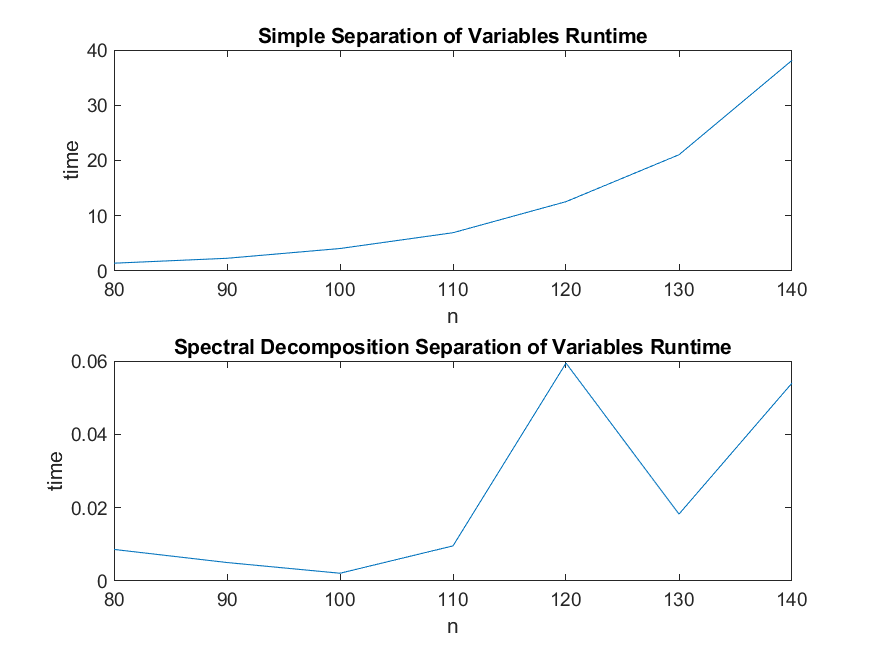
\includegraphics[width=0.5\textwidth]{runtime_dif.png} & 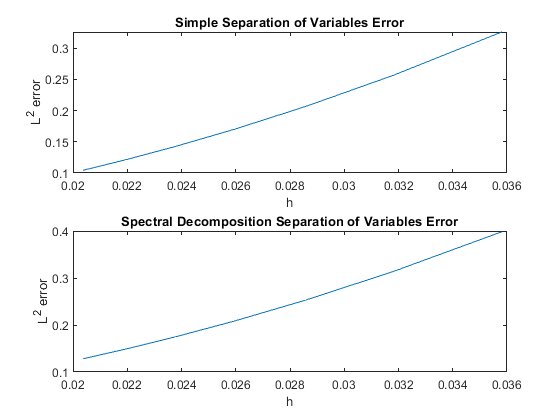
\includegraphics[width=0.5\textwidth]{error_dif.png}\\
\bottomrule
\end{longtable}

\newpage
From the results we decided to go with the discrete separation of
variables approach.

Additionally, we did some test runs for different values of the wave
number \(k\), to study the behaviour of our model.

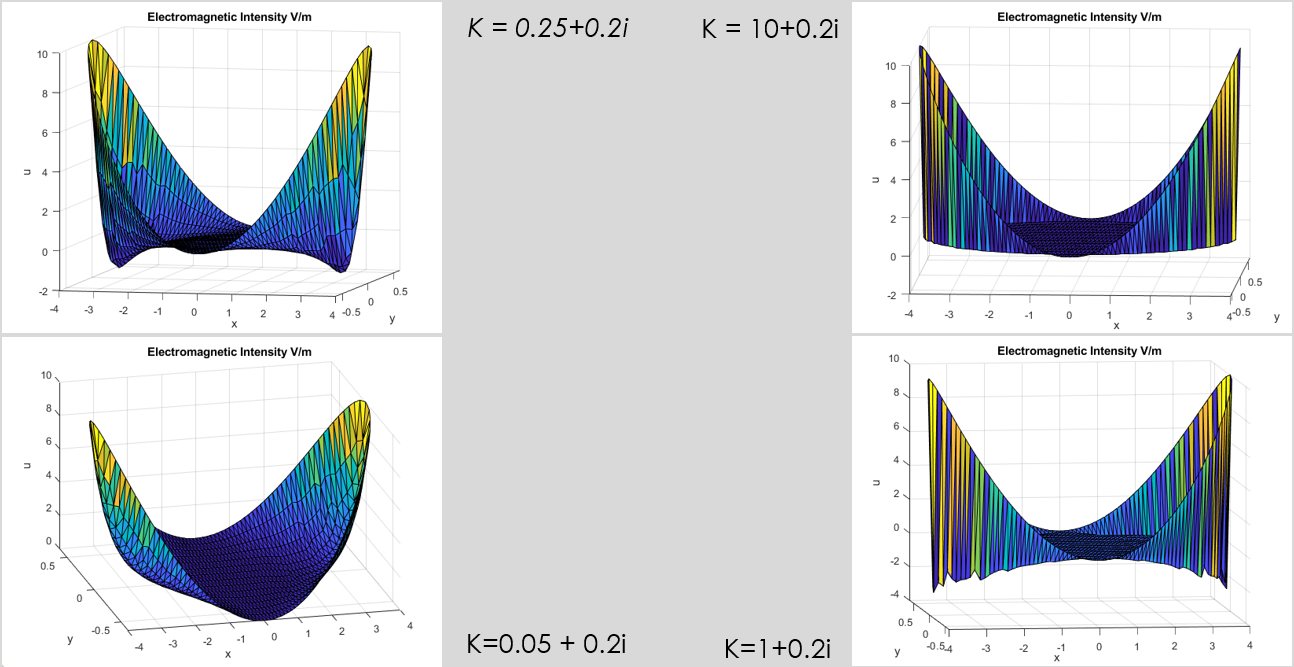
\includegraphics[width=\linewidth]{kvalsellip.png}

\section{Results}

Using the equations and parameters described in the previous sections,
we arrived at the following results for our two regions of interest
i.e. a rectangular bus bar and an elliptical one. Firstly, we concluded
that the electromagnetic intensity is greater at the end points, and
decays in the midsections of the copper bus bar as shown in the figures
below. This implied that our models adequately represent a real world
scenario of the problem according to our discussion with our industry
mentor at McGillan-McGee. Additionally, we would like to mention that
from the two chosen regions used for our models, the rectangular bus bar
is more applicable as it is most resembles the real world situation;
since this is most common shape of bus bars. The elliptical model
results will allow our industry partner at McGillan-McGee to continue
investigating the work done by McLachlan$^1$ on the subject, which was
the original problem that was presented to us. It is important to remark
that our models are generalized so it is trivial to substitute the
parameters for alternative conditions.
\newpage
\begin{longtable}[]{@{}ll@{}}
\toprule
Rectangular & Elliptical \\
\midrule
\endhead
& \\
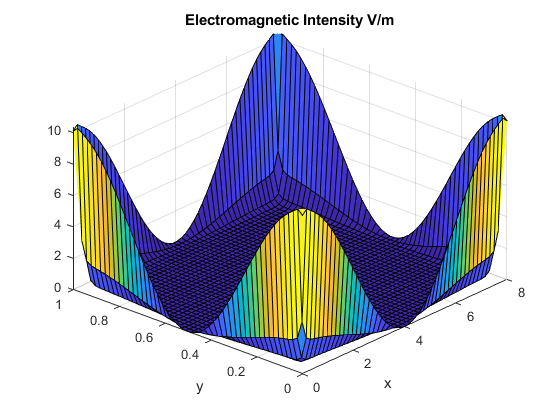
\includegraphics[width=0.5\textwidth]{rect.png} & 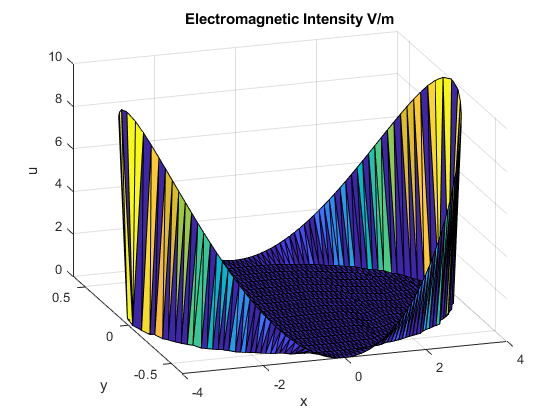
\includegraphics[width=0.5\textwidth]{ellip.png}\\
\bottomrule
\end{longtable}

\section{Conclusions}

Having created the rectangular model that accurately depicts the
scenario of current flowing through a copper bus bar, Maxwells Equations
can be used to characterize resistance and inductance. Knowing the
resistance and inductance will allow McGillan-McGee to alter the copper
bus bar in such a way that voltage spikes will not run back through it
and ruin the attached machinery. The elliptical model we created will
allow McGillan-McGee to continue following along McLachlan's\(^1\) work
and potentially pursue a different avenue.

\section{Acknowledgements}

We would like to express our deep gratitude to our terrific mentor, Dr. Shaun Lui, for his time and wisdom.
Shaun has done a terrific job of introducing us to the right materials that we needed in order to endeavour on our problem.
We would also wish to thank  our industry mentor, Edwin Reid, for the opportunity to work on this project with him
and  for his eagernes to share his industry expertise. Finally, we want to thank the organizers of the PIMS $Math^{Industry}$ workshop, 
especially to Professors Allen Herman and Kristine Bauer for their support. 

\section{References}

{[}1{]}: Norman W. McLachlan, ``Theory and Applications of Mathieu
Functions'', Oxford University Press, 1947.

{[}2{]}: S. H. Lui, 'Numerical Analysis of Partial Differential Equations', Wiley, 2011

\newpage

\section{Appendix}
\includepdf[pages=-]{Equations1.pdf}


    % Add a bibliography block to the postdoc
    
    
    
\end{document}
